
\tolerance=1
\emergencystretch=\maxdimen
\hyphenpenalty=10000
\hbadness=10000

\documentclass[a4paper,12pt]{article}		
\usepackage[brazilian]{babel}
\usepackage[T1]{fontenc}
\usepackage{avant}
\usepackage[utf8]{inputenc}
\usepackage{float}
\usepackage{graphicx}
\usepackage[dvipsnames]{xcolor}
\usepackage{titling}
\usepackage{wrapfig}
\usepackage{indentfirst}
\usepackage[left=2cm, right=2cm, top=1cm, bottom=2cm, includeheadfoot, headheight=2cm]{geometry}
\usepackage{makeidx}   
\usepackage{wallpaper}      							% índice remissivo

\usepackage{listingsutf8}
\usepackage{caption}

% Definindo cores personalizadas para o código
\definecolor{codegreen}{rgb}{0,0.6,0}
\definecolor{codegray}{rgb}{0.5,0.5,0.5}
\definecolor{codepurple}{rgb}{0.58,0,0.82}
\definecolor{backcolour}{rgb}{0.95,0.95,0.92}

% Configuração do estilo do código
\renewcommand{\lstlistingname}{C\'odigo} % Muda "Listing" para "Código"
\lstset{
    language=C++,                          
    backgroundcolor=\color{backcolour},   % Cor de fundo
    commentstyle=\color{codegreen},       % Cor dos comentários
    keywordstyle=\color{magenta},         % Cor das palavras-chave (void, int, if)
    numberstyle=\tiny\color{codegray},    % Estilo dos números das linhas
    stringstyle=\color{codepurple},       % Cor do texto entre aspas
    basicstyle=\ttfamily\small,           % Fonte monoespaçada para o código
    breakatwhitespace=false,              
    breaklines=true,                      % Quebra a linha automaticamente se o código for longo
    captionpos=b,                         % Legenda na parte inferior
    keepspaces=true,                      % Mantém os espaços/indentação
    numbers=left,                         % Coloca os números das linhas na esquerda
    numbersep=5pt,                        
    showspaces=false,                
    showstringspaces=false,
    showtabs=false,                  
    tabsize=2,
    inputencoding=utf8/latin1
}

\makeatletter
\makeatother

\usepackage[
    colorlinks=true,        % Ativa a cor apenas no texto, sem bordas
    linkcolor=black,        % Links internos (figuras, sumário) ficam pretos
    urlcolor=magenta]
{hyperref}


 
\usepackage{fancyhdr}                              		% Para uso de cabeçalhos e rodapés
\setlength{\headheight}{70pt}
\definecolor{light-gray}{gray}{0.30}					% Definição de cor em escala de cinza por porcentagem
\definecolor{azulpetroleo}{RGB}{64,128,128}
\definecolor{laranja}{RGB}{255,127,0}
\definecolor{verde-uel}{RGB}{0,119,1}

\fancypagestyle{RAMOIEEE}{		                        
% Estilo do Tema para cabeçalhos e rodapés - Nome do tema
\renewcommand{\headrulewidth}{2pt} 						
% Estilo do Tema para cabeçalhos e rodapés - Espessura da linha no cabeçalho
\renewcommand{\footrulewidth}{2pt} 						
% Estilo do Tema para cabeçalhos e rodapés - Espessura da linha no rodapé
\renewcommand{\headrule}{{\color{black}          		
% Muda as regras da linha no cabeçalho
\hrule width\headwidth height\headrulewidth \vskip-\headrulewidth}}		
\renewcommand{\footrule}{{\color{black}					
% Muda as regras da linha no rodapé
\vskip-\footruleskip\vskip-\footrulewidth																	
\hrule width\headwidth height\footrulewidth\vskip\footruleskip}}}


\begin{document}

%% => -------------------------------------------------Configurações do Papel Timbrado

\pagestyle{RAMOIEEE}	 													
% Habilita o uso de cabeçalhos e rodapés no tema configurado
\lhead{
\includegraphics[height = 2cm]{../figs_template/ieeelogo1pb.jpg}\vspace{0.3cm}}		
% Coloca uma figura no cabeçalho à esquerda (left)
\chead{{\LARGE \bf Ramo Estudantil IEEE - UEL}\vspace{1.0cm}} 				
% Coloca um texto no centro (center) cabeçalho
\rhead{
\includegraphics[height = 2cm]{../figs_template/logouel.jpg}\vspace{0.3cm}}
\fancyfoot{} 																
% Limpa o rodapé. É para garantir que não terá nada no rodapé.
\cfoot{{\small Contato do Ramo: sb.uel@ieee.org }\\{\small Institute of Electrical and Electronics Engineers - IEEE}\\{\small Universidade Estadual de Londrina - UEL $\bullet$ Paraná - Brasil}} 
% Coloca um texto no centro (center) do rodapé						

%% => -------------------------------------------------Fim das Configurações do Papel Timbrado

%% => -------------------------------------------------Início do texto

\begin{titlepage} 
\thispagestyle{RAMOIEEE}

\begin{center}
 
    \vspace{30pt}
        
	\fbox{\textbf{Gestão}} \\
            \vspace{5pt}
            \textbf{Presidente:} Marco Antônio C. Henry \\
            \textbf{Vice-Presidente:} Nicolas Oliveira \\
            \textbf{Líder do Projeto:} Ashley de Farias Bonassoli \\
            

    \vspace{15pt}

    \fbox{\textbf{Relatório mensal}} \\
    \vspace{5pt}
            
            \large{\textbf{Alimentador de Rua Inteligente}} \\

    \vspace{66pt}


    \begin{figure}[h]
    \centering
    
\includegraphics[width=0.8\textwidth]{../figs/IEEE-CS_LogoTM-orange.png}
    \end{figure}

\end{center}

\vspace{80pt}

\fbox{\textbf{Integrantes}} 
\begin{itemize}
    \item Ashley de Farias Bonassoli
    \item Gabriela Siqueira Loiola
    \item Ana Vitória Machado
    \item Osvaldina Dias
\end{itemize}

\begin{flushright}
    \fbox{\textbf{Redação}} \\
    \vspace{5pt}
    Ashley de Farias Bonassoli
    
\end{flushright}

\end{titlepage}

\newpage

\title{Abril}
\date{}
\author{}
\maketitle
\vspace{-1.4cm}

Utilizamos o site \href{https://www.tinkercad.com}{Tinkercad} para nos familiarizarmos com a montagem do circuito. Nele, é possível criar um ambiente virtual no qual é possível testar ligações entre Arduino, resistores, lâmpadas, botões e outros componentes. Além disso, permite escrever e executar códigos em C\texttt{++}, proporcionando maior complexidade e possibilidades aos circuitos.\\

\subsubsection*{Prática realizada}
\noindent Criar um circuito com dois LEDs e dois botões.\\
\vspace{-0.2cm}
\begin{itemize}
    \item Apertar o botão 1 $\rightarrow$ LED 1 acende, LED 2 apaga
    \item Apertar o botão 2 $\rightarrow$ LED 2 acende, LED 1 apaga
\end{itemize}

\begin{figure}[h]
    \centering
    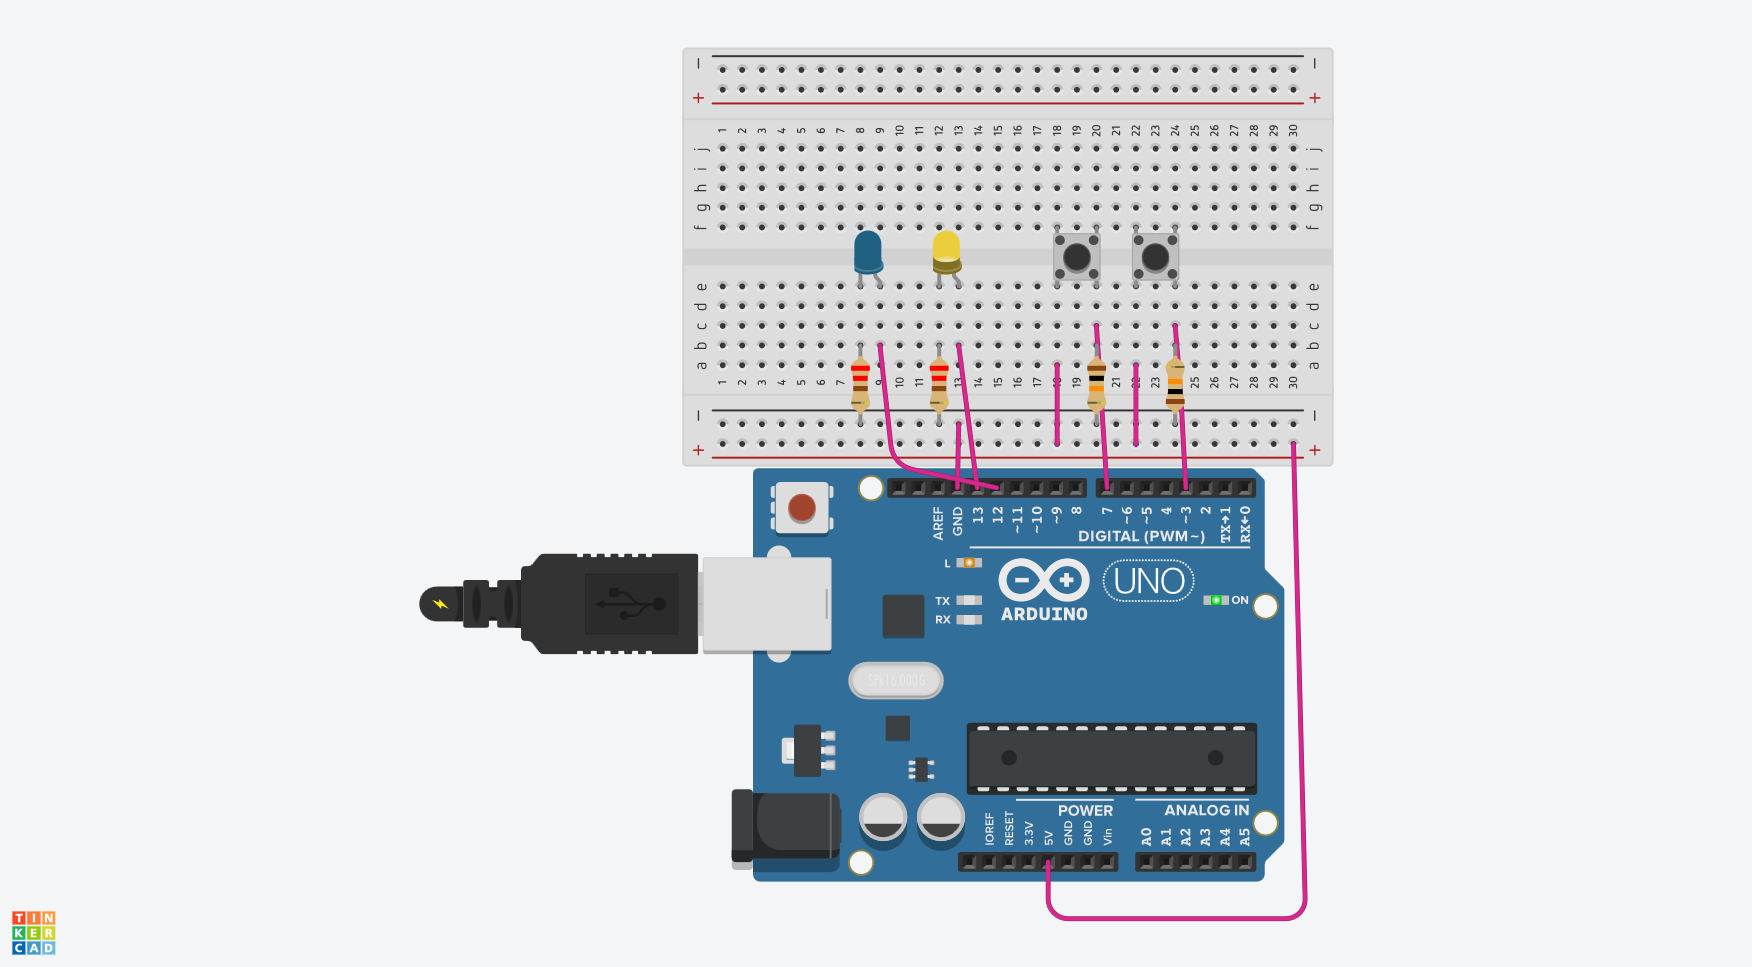
\includegraphics[width=1.0\textwidth]{../figs/pratica-arduino.png}
    \caption*{Circuito montado no Tinkercad.}
    \label{fig:circuito_arduino}
\end{figure}

\newpage

\lstinputlisting[title={C\'odigo-fonte do programa do Arduino}]{../codes/pratica_arduino.ino}
\bigbreak

\noindent Circuito no Tinkercad: \href{https://www.tinkercad.com/things/isqw31TJhYH-pratica-dois-botoes?sharecode=OD8YmILx-zFJkZS_fJNu8jKlsnR4dTg6y4rJ6c_sYVA}{Prática - dois botões} \\
\noindent Material de apoio utilizado: \href{https://www.blogdarobotica.com/2020/09/28/ligar-e-desligar-led-com-botao-push-button-chave-tactil-com-arduino/}{Blog da Robótica}.


\end{document}